\newpage
\section{Internal consistency}
\label{Internal_consistency}
When generating a topic model with \ac{LDA} or \ac{NMF} the number of topics has to be manually set. This number is critical and has an effect on the quality and the interpretability of topics. We want to provide the domain experts an overview how topics change when increasing or decreasing the topic number. So they can assess, which topic model is the appropriate one for their further research. 

To analyze the quality of a topic model we differentiate between the intra topic model and inter topic model approach. The intra topic approach compares all topics of one topic model with each other. This way we can study, which topics are similar to each other or which topics appear together in the same document. When applying the inter topic approach, we compare the topics from topic model A to a second different topic model B. The second topic model differs from the first by the number of topics. By comparing the two models we can study what effect the increasing topic number has on the quality of the topics. With both approaches we want to examine questions such as: Do the topics get more specific, more general, do they split up or do they stay the same and only new topics are added? Are there a few topics, which are dominating in a document or are few topics assigned to a document? How does the topic assignment change across different topic models? Indicates a higher topic number a better clustering of the documents?

Both, \ac{LDA} and \ac{NMF} return a document topic matrix $\theta$, which describes to what extend a topic appears in a document and a topic term matrix $\phi$, which describes to what extend a term appears in a topic. Different key figures can be derived from these matrices to judge the quality and to examine the changes in topics.
Entropy and Jensen Shannon divergence can be used on the document topic matrix as well on the topic term matrix. The coherence measure relies solely on the topic term matrix and alpha $\alpha$  can only be applied on topic models, that were generated with \ac{LDA}.

For our evaluation we generated topic models with 25, 50, 75 topics and topic models with 50 topics over and under the topics number from \textit{Generation 1}. The different key figures were applied on these newly generated topic models and the topic models from \textit{Generation 1}.In the following the dataset for \text{German editorial articles} with 25, 50, 75, 140, 190 and 240 topics per topic model were analyzed.

\subsection{Theta $\theta$}
\begin{table}[h]
	\centering
	\begin{tabular}{c|ccccc}
		&Topic 1&Topic 2&Topic 3&Topic 4&Topic 5\\
		\hline
		Document 1&0.1 & 0.4 & 0.05 & 0.25 & 0.2  \\
		Document 2&0.025&0.8 & 0.025 & 0.07 & 0.03\\
	\end{tabular}
	\caption[Document topic matrix]{Example for a document topic matrix}
	\label{doc_topic}
\end{table}
The document topic matrix $\theta$ describes to which extend a topic is represented in a certain document.
We used the matrix to calculate the number of documents, which are assigned to a topic and the number of topics, which are assigned to a document. In both cases a threshold fo 10\% was used. The example document topic matrix in Table \ref{doc_topic} shows two documents and 5 topics. For topic 1 the counter number of documents is only 1 (Document 1). For Document 1 the relevant number of topics is 4 (Topic 1,2,4,5). 

\subsection{Alpha}
Alpha $\alpha$ is a prior parameter for \ac{LDA}, that describes the sparsity of the topic distribution for every document. Usually, the prior $\alpha$ has to be set and has the same value for every topic. In this case it is called the symmetric Dirichlet prior. However, \cite{Blei2003} showed how $\alpha$ can be estimated from the data per topic. In this case $\alpha$ is an asymmetric Dirichlet prior. This method was used for our topic model, to determine how important the topics are for the whole corpus. A high $\alpha$ value means that the documents are mixtures of many topics, while a low $\alpha$ value means, that the documents are composed of only a few highly probable topics (\cite{Steyvers2007}).

In Figure \ref{alpha_dist} the alpha values for each topic for German editorial articles with 190 topics are shown. The document distribution for Topic 30, which has the lowest alpha value, is considered in Figure \ref{alpha_min}. The x-axis represents the document ids, standing for the documents, which build the corpus. The y-axis represents the percentage of a document that is covered by the topic. In contrast to Topic 30, Topic 111 with the highest alpha value is shown in Figure \ref{alpha_max}. One can see, that Topic 30 covers only a few documents, while Topic 111 is more evenly spread over all documents.

%%beispiel für alpha
\begin{figure}[t]
	\centering
	\subfloat[Plotted alphas for German editorial articles]{\label{alpha_dist}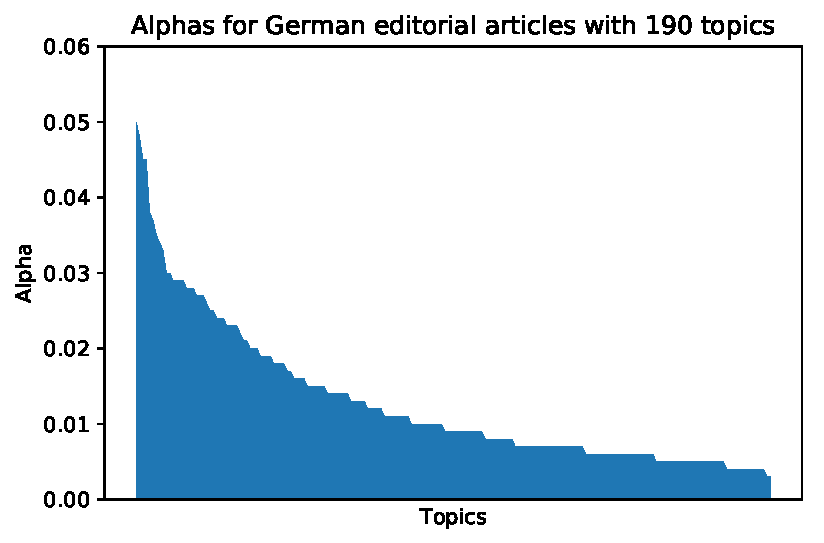
\includegraphics[width=8cm]{gfx/Alphas/German_editorial_articles_with_190_topics_100.pdf}}\par\medskip
	\begin{minipage}{0.5\textwidth}
		\centering
		\subfloat[Document coverage for the topic with the lowest alpha value ]{\label{alpha_min}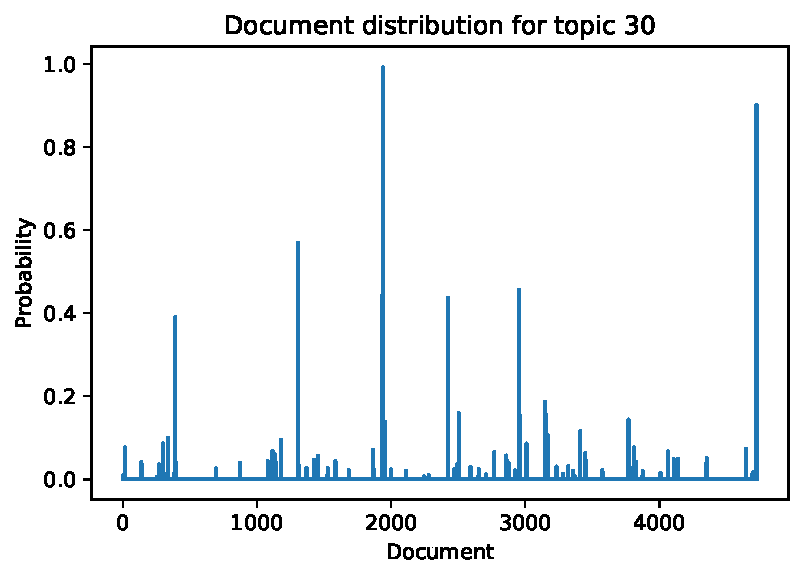
\includegraphics[width=7cm]{gfx/doc_topic_max_min/German190t30.pdf}}
	\end{minipage}%
	\begin{minipage}{0.5\textwidth}
		\centering
		\subfloat[Document coverage for the topic with the highest alpha value]{\label{alpha_max}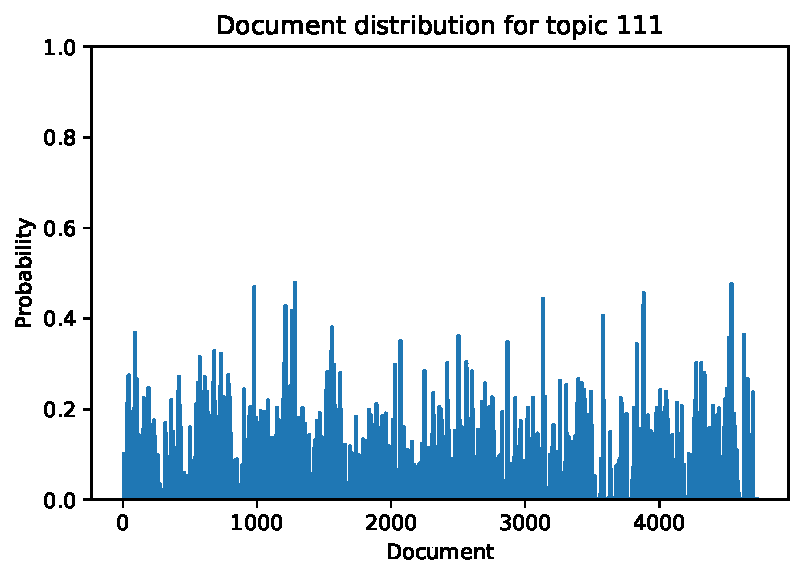
\includegraphics[width=7cm]{gfx/doc_topic_max_min/German190t111.pdf}}
	\end{minipage}
	\caption[]{Alpha values for German editorial articles with 190 topics and the topic document matrices for the topic with the highest and lowest alpha value}
	\label{alpha_example}
\end{figure}

\subsection{Entropy}
Entropy was used to identify specific and general topics. It can be applied on the topic term matrix $\phi$ and the document topic matrix $\theta$. When applied on the topic term matrix, a high entropy value indicates that the topic is rather general. This means, that all terms have a similar probability to appear in the topic. A low entropy indicates, that the topic is specific i.r. only a few words have a high probability to appear in the topic. This difference is illustrated in Figure  \ref{entropy_min} and in Figure \ref{entropy_max}. \newline
When applied on the document topic matrix $\theta$ the rules can be applied analogously. A high entropy value indicates, that the topic is rather general. This means, that all topics have a similar probability to appear in a document. A low entropy value indicates, that the topic is specific i.e. only a few topics have a high probability to appear in a document. Entropy is calculated as follows (\cite{Sethi2012}):
\begin{equation}
E = -\sum(p * log(p))
\end{equation}
where $p$ is the probability of a term in a topic, which was taken from the topic term matrix $\phi$ or the probability of a topic in a document, taken from the document topic matrix $\theta$. 
In Figure \ref{entropy_dist} the entropy values for each topic for German editorial articles with 190 topics are shown. The entropy values are sorted descending. The topic term matrix for Topic 13, which has the lowest entropy value, is considered in Figure \ref{entropy_min}. The x-axis represents each termid of the corpus. The y-axis represents the probability of the terms in a topic. In contrast to Topic 13, Topic 100 with the highest entropy value is shown in Figure \ref{entropy_max}. One can see, that Topic 13 consists mainly of the term id 4916 and the other term ids hardly occur, while in Topic 100 the term ids are nearly evenly spread.
\begin{figure}[t]
	\centering
	\subfloat[Plotted entropy for German editorial articles]{\label{entropy_dist}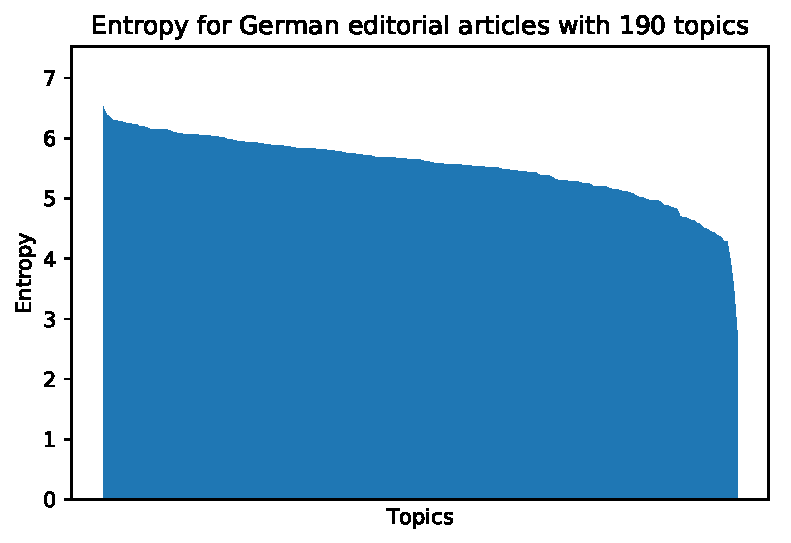
\includegraphics[width=7cm]{gfx/Entropy/German_editorial_articles_with_190_topics100.pdf}}\par\medskip
	\begin{minipage}{0.5\textwidth}
		\centering
		\subfloat[Topic coverage for the topic with the lowest enropy ]{\label{entropy_min}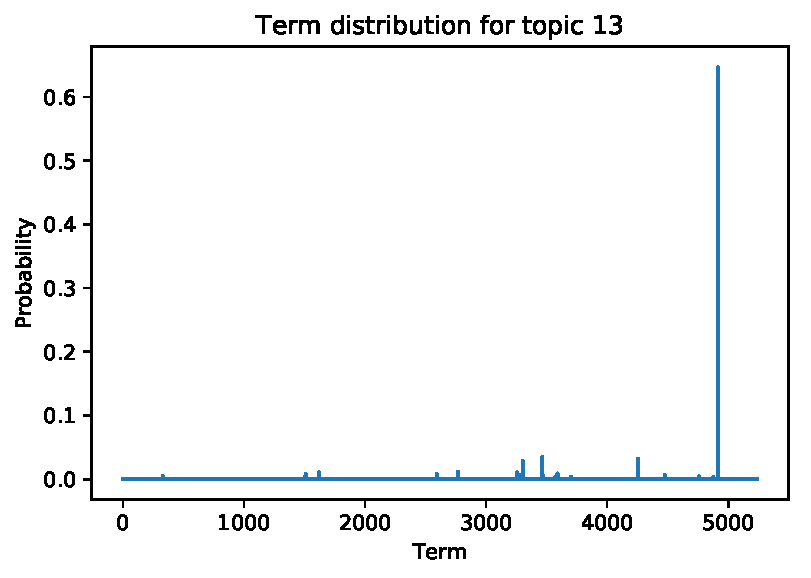
\includegraphics[width=6.65cm]{gfx/topic_term_max_min/German190t13.pdf}}
	\end{minipage}%
	\begin{minipage}{0.5\textwidth}
		\centering
		\subfloat[Topic coverage for the topic with the highest entropy ]{\label{entropy_max}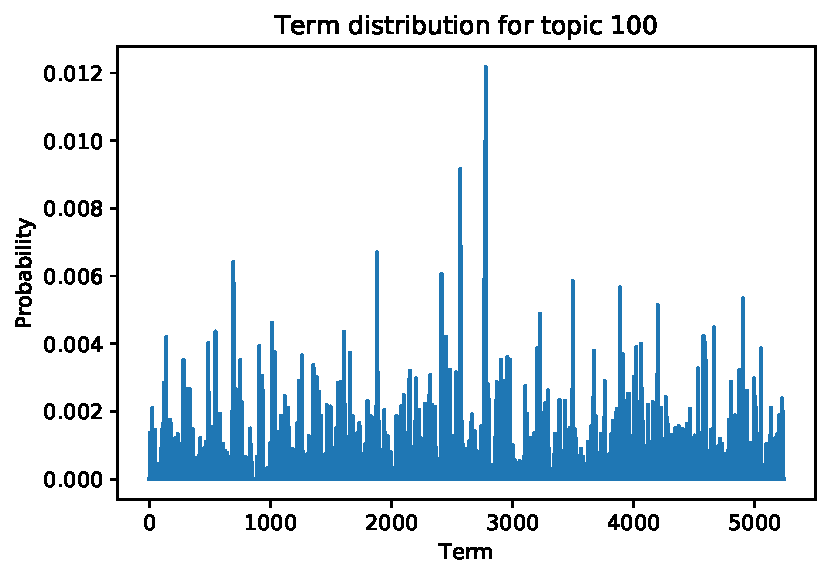
\includegraphics[width=7cm]{gfx/topic_term_max_min/German190t100.pdf}}
	\end{minipage}
	\caption[]{Entropy for German editorial articles with 190 topics and the topic term matrices for the topic with the highest and lowest entropy}
	\label{entropy_example}
\end{figure}


\subsection{Coherence}
The coherence scores topics by measuring the degree of semantic similarity between words in a topic. This measurement helps to distinguish topics, that are semantically similar and easy interpretable for humans and those that are semantically dissimilar and not easy interpretable.(\cite{Stevens2012}) There are different coherence measure such as the UCI-measure (\cite{Newman2010}) and the U-mass measure(\cite{Mimno2011}). Both measure the coherence of a topic as the sum of pairwise distributional similarity scores over a set of topic words:
%Both measures compute the coherence of a topicas the sum of pairwise distributional similarity scores over the set of topic words, V .
\begin{equation}
coherence (V) = \sum_{v_{i},v_{j}\in V} score(v_{i},v_{j})
\end{equation}
$V$ describes the set of words for a topic, while $v$ is a single word, occurring in a topic. We used the top-10 words of a topic to calculate the coherence score for each topic in a topic model.
We used the UMass metric, which is based on the document co-occurrence and defined as: 
\begin{equation}
socre(v_{i},v_{j}) = log\frac{D(v_{i},v_{j})+1}{D(v_{j})}
\end{equation}
$D(v_{j})$ is the document frequency, that count the number of documents which include the word $v_{j}$. $D(v_{i},v_{j})$ is the co-document frequency, that counts the documents, which include both word $v_{i}$ and $v_{j}$. A smoothing count of 1 is included to avoid taking the logarithm of zero. The UMass metric computes these counts over the original corpus, which was used to train the topic models (\cite{Stevens2012}). The coherence score is negative and the higher interpretability of a topic is given with a score near to zero.

\subsection{Jensen Shannon divergence}
The topics returned by \ac{LDA} are probability distributions over all terms in the corpus. Therefore, to compare the similarity of two topics $p$ and $q$ we can use existing metrics to measure the similarity between probability distribution. \cite{Lin1991} et al lists possible similarity functions. A standard function to measure the difference or divergence between two probability distributions $p$ and $q$ is the Kullback Leibler (\ac{KL}) divergence:
\begin{equation}
	D(p,q) = \sum_{j=1}^{T} p_{j} log_{2} \frac{p_{j}}{q_{j}}
\end{equation}
 where $j$ is the number of a certain term and $T$ describes the total number of terms. $p_{j}$ represents the probability of term $j$ appearing in topic $p$. $q_{j}$ is the probability of term $j$ appearing in topic $q$. The \ac{KL} divergence is an asymmetric measurement. For our use-case, comparing the topics intra and inter a topic model, a symmetric measure is needed, which guarantees the same results for the comparison of $t1$ with $t2$ and $t2$ with $t1$. Therefore, based on the \ac{KL} divergence, the \ac{JS} divergence is used:
\begin{equation}
	JS(p,q)  = 0.5 * (D(p,\frac{p + q}{2}) + D(q, \frac{p + q}{2}) )
\end{equation}
The \ac{JS} divergence  is a symmetric extension of the \ac{KL} divergence. If the probability distributions are identical, the value 0 is assigned otherwise the value 1 is assigned for totally dissimilar probability distributions (\cite{Steyvers2007}).
In our implementation we subtracted the value from the \ac{JS} divergence from 1 to get the similarity between two probability distributions, so that the value 1 is assigned when two probability distributions are identical and the value 0 when they are completely dissimilar. 

\subsection{Evaluation}
The evaluation was conducted on \textit{German} and \textit{English editorial articles}. For both datasets we studied topic model with 50 topics over and under the optimal topic number from \textit{Generation 1} and further generated topic models with 25, 50 and  75 topics. Both datasets were analyzed by applying each key figure as explained above on each topic model. The results per key figure and per topic model were then compared with each other.
\subsubsection{Entropy}
%%%German
\begin{figure}
	\begin{minipage}{0.5\textwidth}
		\centering
	\begin{tabular}[t]{c|cc}
		&max value & min value\\
		\hline
		25 topics&7.08&5.42\\
		50 topics&	6.82&4.67\\
		75 topics&	6.79&4.40\\
		140 topics&	6.60&3.99\\
		190 topics &6.52&2.78\\
		240 topics&	6.57&3.09\\
	\end{tabular}
	\end{minipage}%
	\begin{minipage}{0.5\textwidth}
		\centering
		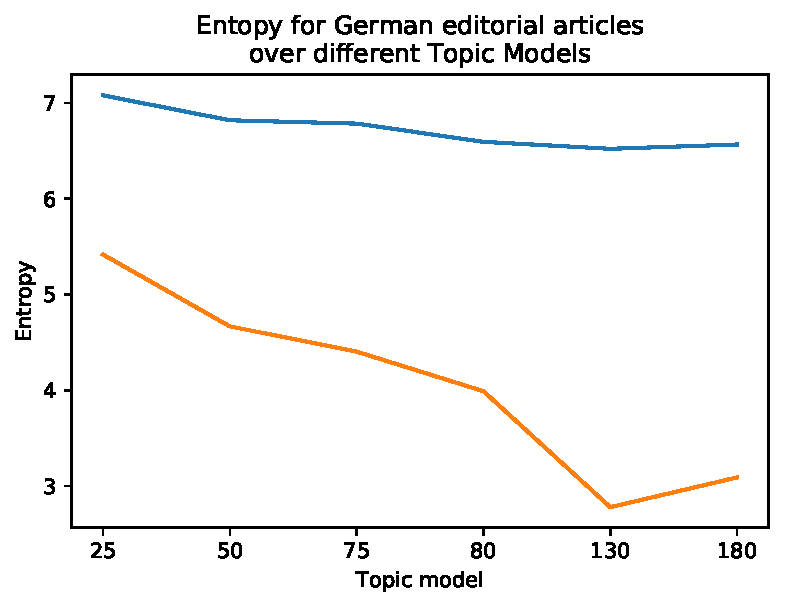
\includegraphics[width=7cm]{gfx/Eval_IC/German_Editorial_Entropy.pdf}
	\end{minipage}
	\caption{Maximal and minimal entropy per topic model for German editorial articles.}
	\label{entr_german}
\end{figure}
%%%English
\begin{figure}
	\begin{minipage}{0.5\textwidth}
		\centering
		\begin{tabular}[t]{c|cc}
			&max value & min value\\
			\hline
			25 topics&7.029&5.455\\
			50 topics&6.8&4.71\\
			75 topics&6.823&4.636\\
			80 topics&	6.819&4.112\\
			130 topics & 8.741&4.005\\
			180 topics&	8.741&3.249\\
		\end{tabular}
	\end{minipage}%
	\begin{minipage}{0.5\textwidth}
		\centering
		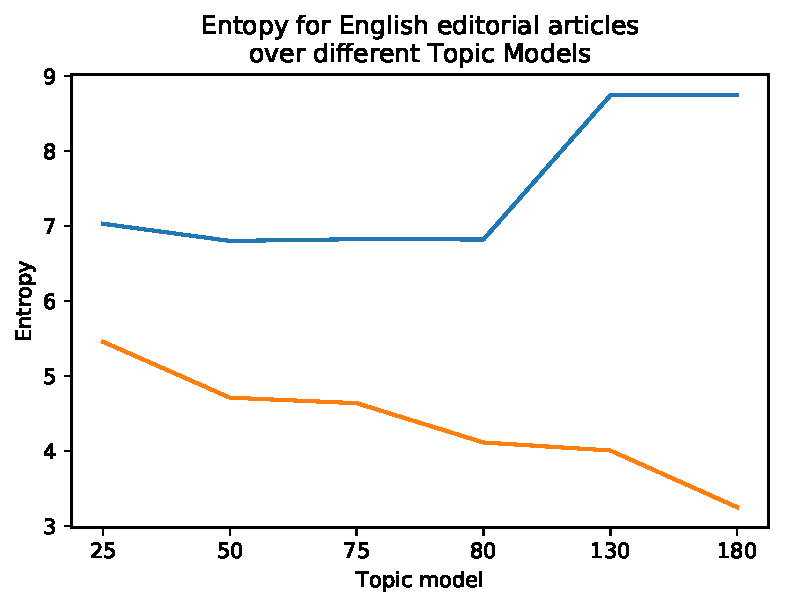
\includegraphics[width=7cm]{gfx/Eval_IC/English_Editorial_Entropy.pdf}
	\end{minipage}
	\caption{Maximal and minimal entropy values per topic model for English editorial articles.}
	\label{entr_english}
\end{figure}
The Figures \ref{entr_german} and \ref{entr_english} show the change of entropy for \textit{German} respectively \textit{English editorial articles}. The table on the left denotes the minimal and maximal entropy given the number of topics. On the right the maximal entropy values (blue line) and the minimal entropy values (orange line) are plotted. This structure will repeat in the different key figures.

The entropy values for \textit{German editorial articles} (Figure \ref{entr_german}) are decreasing when increasing the number of topics. For the topic model with 240 topics the entropy values starts increasing again. This means, that the topics with a higher topic number are getting more specific until a certain point, when the entropy value is increasing again. This could mean, that the optimal topic number, to generate topics, which are specific, is at the point, when the entropy value has reached its minimum.

For \textit{English editorial articles} (Figure \ref{entr_english}) the maximal entropy value is decreasing up to the topic model with 80 topics. Then the values is rising and for the topic models with 130 and 180 topics the entropy stays the same. For the minimal entropy the values are getting continuously smaller. So the span between the maximal and the minimal entropy value is increasing. This means, that the more topics are generated the more topics get more general and more specific. 

\subsubsection{Alpha}
%%%german editorial
\begin{figure}
	\begin{minipage}{0.5\textwidth}
		\centering
			\begin{tabular}[t]{c|cc}
				&max value & min value\\
				\hline
				25 topics&0.186&0.027\\
				50 topics&0.104&0.015\\
				75 topics&0.065&0.011\\
				140 topics&	0.061&0.004\\
				190 topics &0.050&0.003\\
				240 topics&	0.046&0.002\\
			\end{tabular}
	\end{minipage}%
	\begin{minipage}{0.5\textwidth}
		\centering
		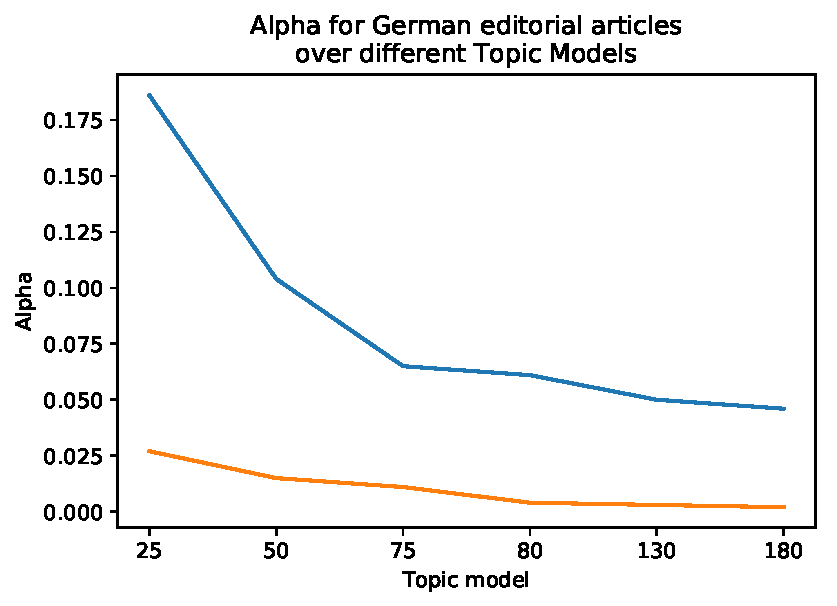
\includegraphics[width=7cm]{gfx/Eval_IC/German_Editorial_Alpha.pdf}
	\end{minipage}
	\caption{Maximal and minimal alpha values per topic model for German editorial articles.}
	\label{alpha_ger}
\end{figure}
%%%english editorial
\begin{figure}
	\begin{minipage}{0.5\textwidth}
		\centering
		\begin{tabular}[t]{c|cc}
			&max value & min value\\
			\hline
			25 topics&0.159&0.032\\
			50 topics&0.229&0.013\\
			75 topics&0.159&0.010\\
			80 topics&	0.180&0.004\\
			130 topics &0.144&0.002\\
			180 topics&	0.118&0.002\\
		\end{tabular}
	\end{minipage}%
	\begin{minipage}{0.5\textwidth}
		\centering
		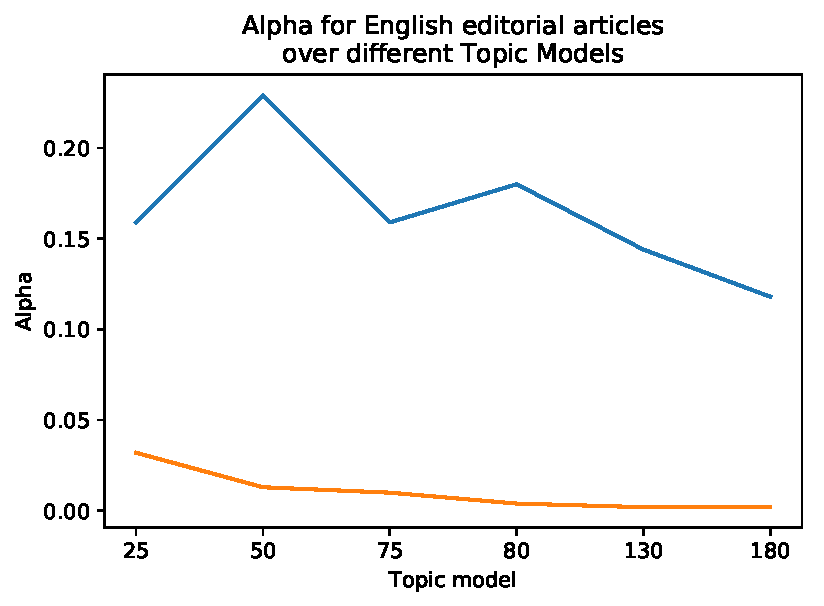
\includegraphics[width=7cm]{gfx/Eval_IC/English_Editorial_Alpha.pdf}
	\end{minipage}
	\caption{Maximal and minimal alpha values per topic model for English editorial articles.}
	\label{alpha_eng}
\end{figure}
In Figure \ref{alpha_ger} the alpha values for \textit{German editorial articles} are shown. The maximal alpha values as well the minimal alpha values are decreasing. This indicates, that the documents are described by fewer topics with a higher probability. But alpha does not say anything about the topic quality, so the few topics, which are assigned to the document can be rather general or specific. Therefore, we calculated the entropy for the topic with the maximal alpha value 0.186 from the topic model with 25 topics and the minimal alpha value 0.002 from the topic model with 240 topics. We got the entropy value of 7.08 for the topic model with 25 topics and the entropy value of 6.28 for the topic model with 240 topics. So the document with the highest alpha value consists out of either general topics and the document with the lowest alpha value out of specific ones. 

The minimal alpha values for \textit{English editorial articles} (Figure \ref{alpha_eng}) are continuously declining up to the topic model with 130 topics. Then the alpha value is staying the same. The maximal alpha values are volatile, so there is no prediction possible, if the values will raise or fall again.

\subsubsection{Coherence}
%% German
\begin{figure}
	\begin{minipage}{0.5\textwidth}
		\centering
		\begin{tabular}[t]{c|cc}
			&max value & min value\\
			\hline
			25 topics&-0.994&-3.957\\
			50 topics&-0.999&-5.605\\
			75 topics&-1.102&-6.792\\
			140 topics&	-0.956&-6.661\\
			190 topics &-0.912&-9.19\\
			240 topics&	-0.948&-7.25\\
		\end{tabular}
	\end{minipage}%
	\begin{minipage}{0.5\textwidth}
		\centering
		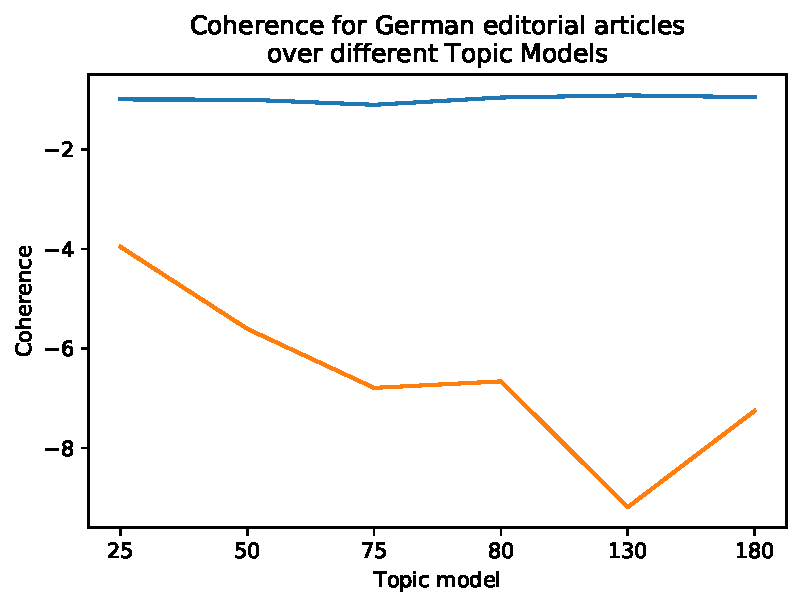
\includegraphics[width=7cm]{gfx/Eval_IC/German_Editorial_Coherence.pdf}
	\end{minipage}
\caption[]{Maximal and minimal coherence values per topic model for German editorial articles.}
\label{eval:coherence_ger}
\end{figure}
	
%% English
\begin{figure}
	\begin{minipage}[t]{0.5\textwidth}
		\centering
		\begin{tabular}{c|cc}
			&max value & min value\\
			\hline
			25 topics&-0.557&-2.242\\
			50 topics&-0.568&-9.570\\
			75 topics&-0.505&-5.913\\
			80 topics&	-0.493&-3.666\\
			130 topics &-0.525&-16.257\\
			180 topics&	-0.549&-16.374\\
		\end{tabular}
	\end{minipage}%
	\begin{minipage}{0.5\textwidth}
		\centering
		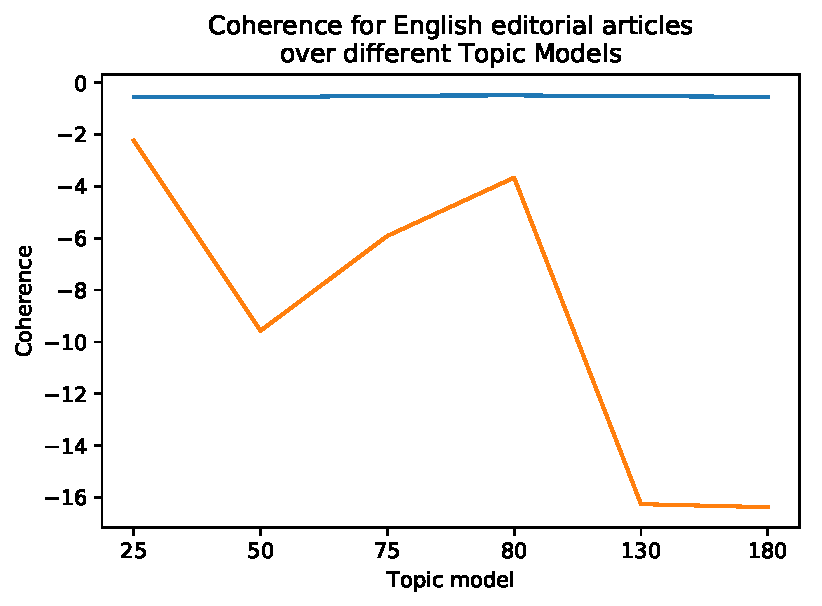
\includegraphics[width=7cm]{gfx/Eval_IC/English_Editorial_Coherence.pdf}
	\end{minipage}
	\caption[]{Maximal and minimal coherence values per topic model for English editorial articles.}
	\label{eval:coherence_en}
\end{figure}
The maximal coherence score is for \textit{German editorial articles} (Figure \ref{eval:coherence_ger}) in the range of the maximal values -0.91 and -1.1 and for \textit{English editorial articles} (Figure \ref{eval:coherence_en}) in the range of -0.49 and -0.56. The maximal values do not change a lot for both datasets, but no pattern how the values are changing can be seen. The same can be said for the minimal coherence values, the only difference is, that the range in which the coherence is moving is much bigger than the range from the maximal values. For \textit{German editorials} it is between -3.96 and -9.2 and for \textit{English editorials} between -2.2 and -16.4.

\subsubsection{Theta}
\begin{figure}
	%german
	\begin{minipage}[t]{0.5\textwidth}
		\centering
		\begin{tabular}{c|cc}
			&max value & min value\\
			\hline
			25 topics&1878&154\\
			50 topics&1026&46\\
			75 topics&693&32\\
			140 topics&655&11\\
			190 topics &423&5\\
			240 topics&	352&5\\
		\end{tabular}
	\end{minipage}
	\begin{minipage}{0.5\textwidth}
	\centering
	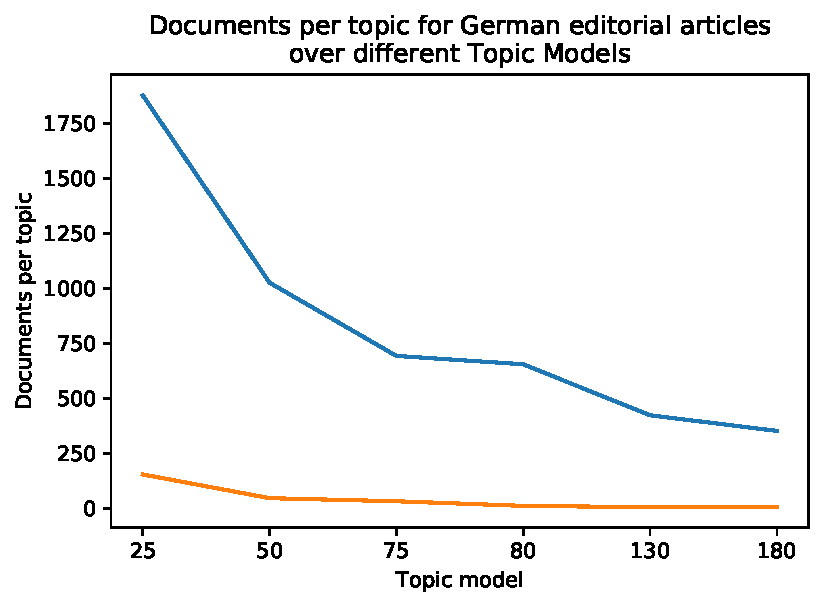
\includegraphics[width=7cm]{gfx/Eval_IC/German_Editorial_Doc_per_topic.pdf}
	\end{minipage}
%english
\caption[]{Maximal and minimal number of documents containing the same topic for German editorial articles.}
\label{eval:amount doc_per_topic_ger}
\end{figure}

\begin{figure}
%english
	\begin{minipage}{0.5\textwidth}
		\centering
		\begin{tabular}[t]{c|cc}
			&max value & min value\\
			\hline
			25 topics&788&58\\
			50 topics&589&13\\
			75 topics&435&7\\
			80 topics&636&7\\
			130 topics &292&0\\
			180 topics&	443&0\\
		\end{tabular}
	\end{minipage}
	\begin{minipage}{0.5\textwidth}
		\centering
		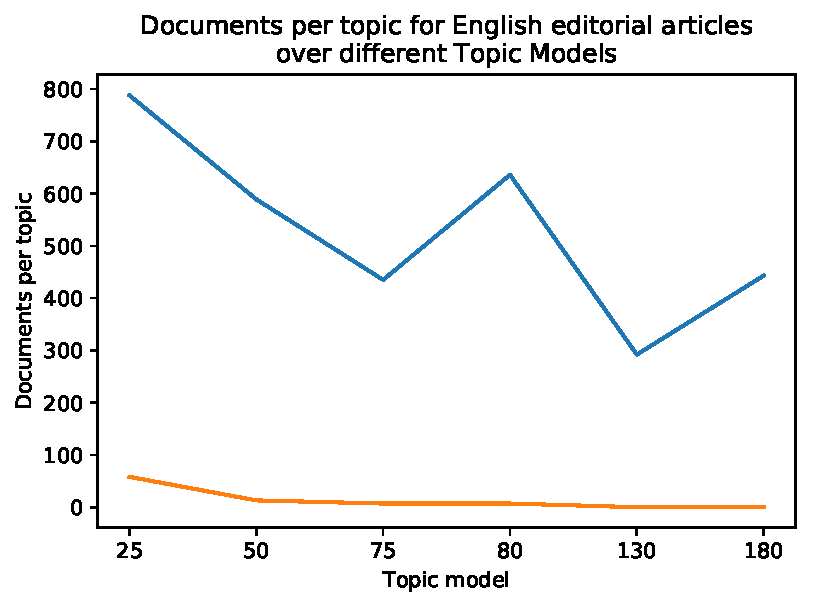
\includegraphics[width=7cm]{gfx/Eval_IC/English_Editorial_Doc_per_topic.pdf}
	\end{minipage}
\caption[]{Maximal and minimal number of documents containing the same topic for English editorial articles.}
\label{eval:amount doc_per_topic_eng}
\end{figure}
In the following we used the document topic matrix to calculate, in how many documents a certain topic covers more then 10\% of the document and how many topics occur over 10\% in a document. 

First, we start with the number of documents a certain topic covers over 10\%.
In Figure \ref{eval:amount doc_per_topic_ger} one can see, that the maximal and minimal number of documents is decreasing when increasing the topic number for \textit{German editorial articles}. This indicated, that the topics are so specific, that they do not appear in any document with a probability higher then the threshold.

For \textit{English editorial articles} (Figure \ref{eval:amount doc_per_topic_eng}) the maximal number of documents is volatile, whereas the minimal numbers of documents are decreasing and there even seem to be topics, that are not assigned to any document, because they do not cover the meaning of the document over the threshold. 

\begin{figure}
	
	\begin{minipage}[t]{0.5\textwidth}
		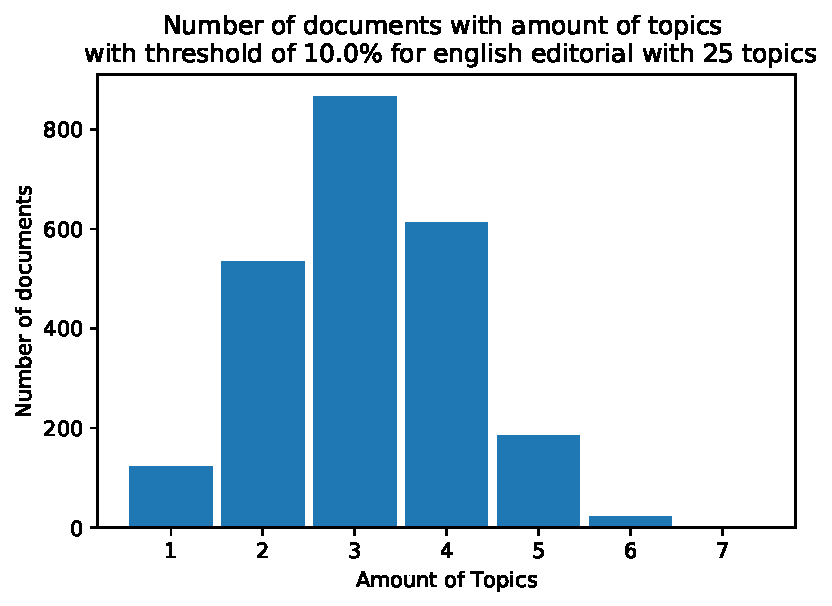
\includegraphics[width=7cm]{gfx/GrafikenFinal/englisheditoriallda_topPerdoc25.pdf}
	\end{minipage}
	\begin{minipage}[t]{0.5\textwidth}
		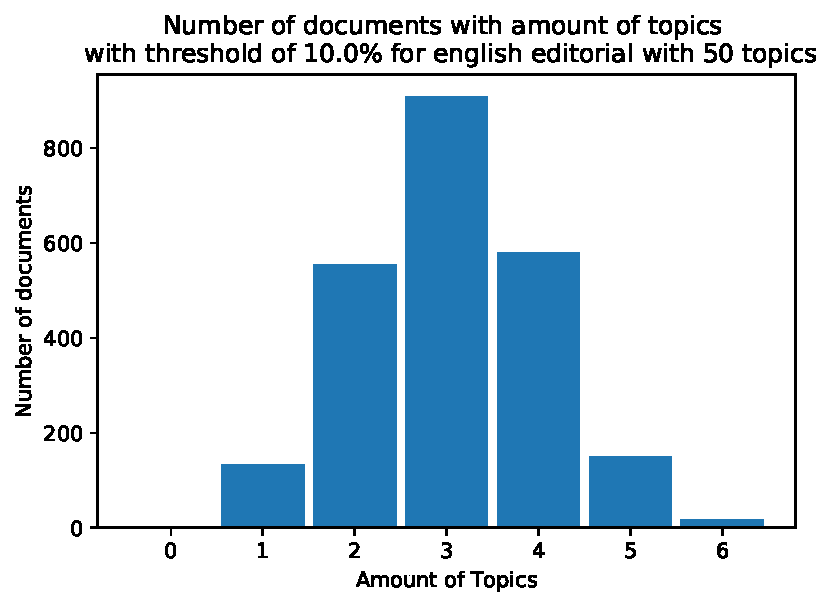
\includegraphics[width=7cm]{gfx/GrafikenFinal/englisheditoriallda_topPerdoc50.pdf}
	\end{minipage}
	\begin{minipage}[t]{0.5\textwidth}
		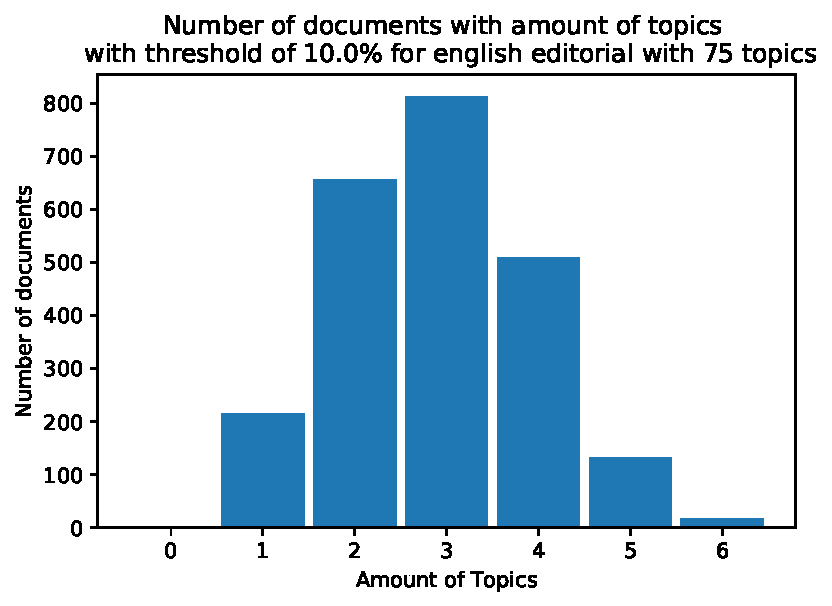
\includegraphics[width=7cm]{gfx/GrafikenFinal/englisheditoriallda_topPerdoc75.pdf}
	\end{minipage}
	\begin{minipage}[t]{0.5\textwidth}
		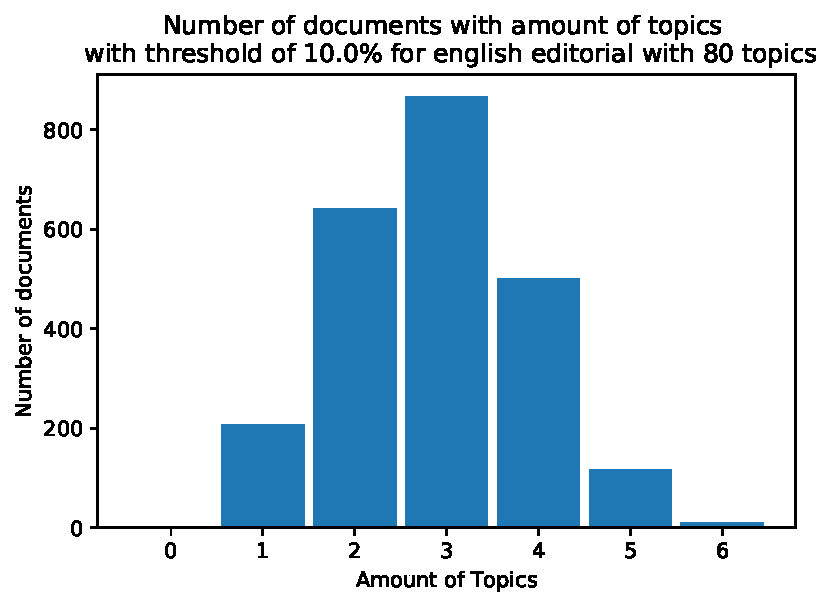
\includegraphics[width=7cm]{gfx/GrafikenFinal/englisheditoriallda_topPerdoc80.pdf}
	\end{minipage}
	\begin{minipage}[t]{0.5\textwidth}
		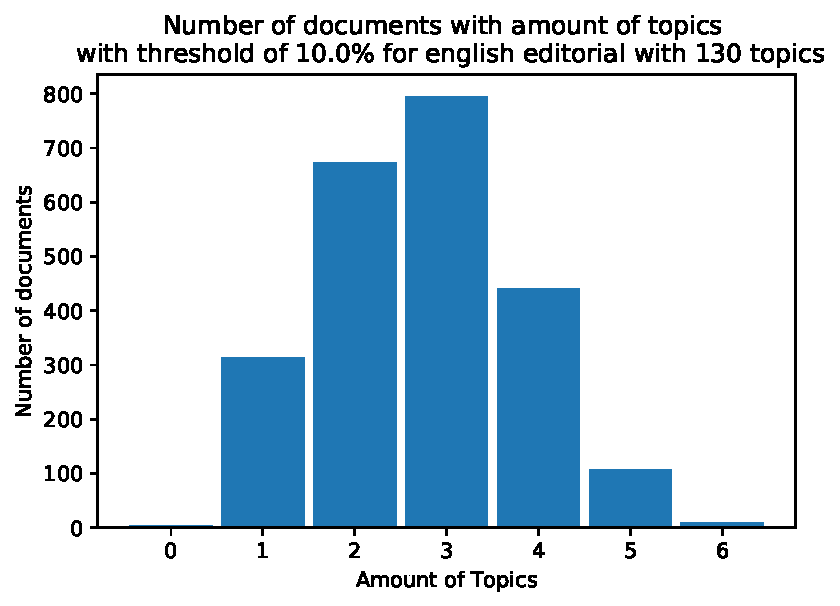
\includegraphics[width=7cm]{gfx/GrafikenFinal/englisheditoriallda_topPerdoc130.pdf}
	\end{minipage}
	\begin{minipage}[t]{0.5\textwidth}
		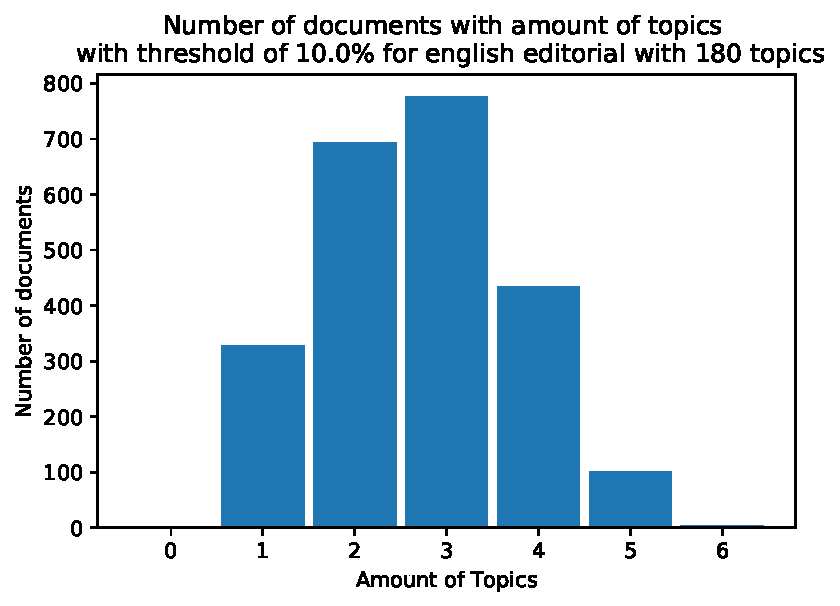
\includegraphics[width=7cm]{gfx/GrafikenFinal/englisheditoriallda_topPerdoc180.pdf}
	\end{minipage}
	\caption{Amount of topics in documents over a threshold of 10\% for English editorial articles}
	\label{top_per_doc_eng}
\end{figure}

\begin{figure}
	\begin{minipage}[t]{0.5\textwidth}
		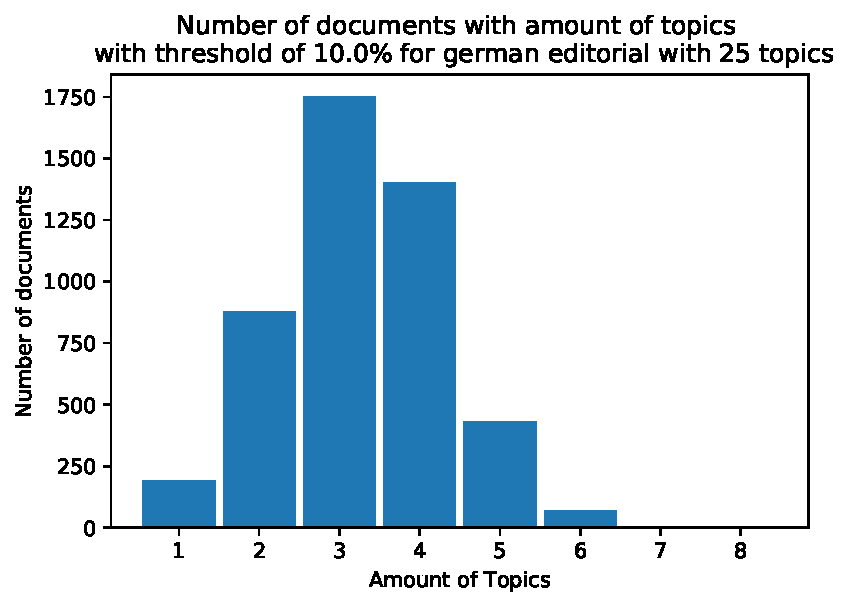
\includegraphics[width=7cm]{gfx/GrafikenFinal/germaneditoriallda_topPerdoc25.pdf}
	\end{minipage}
	\begin{minipage}[t]{0.5\textwidth}
		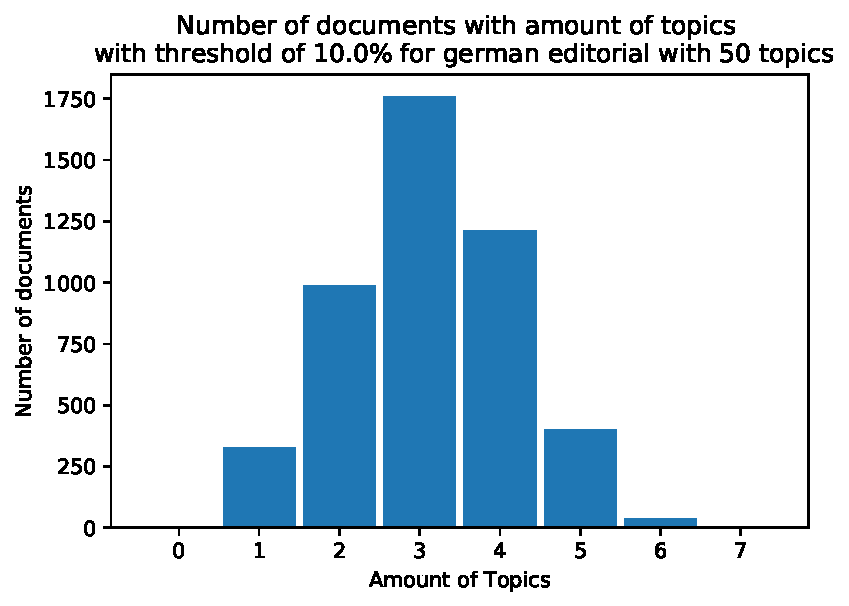
\includegraphics[width=7cm]{gfx/GrafikenFinal/germaneditoriallda_topPerdoc50.pdf}
	\end{minipage}
	\begin{minipage}[t]{0.5\textwidth}
		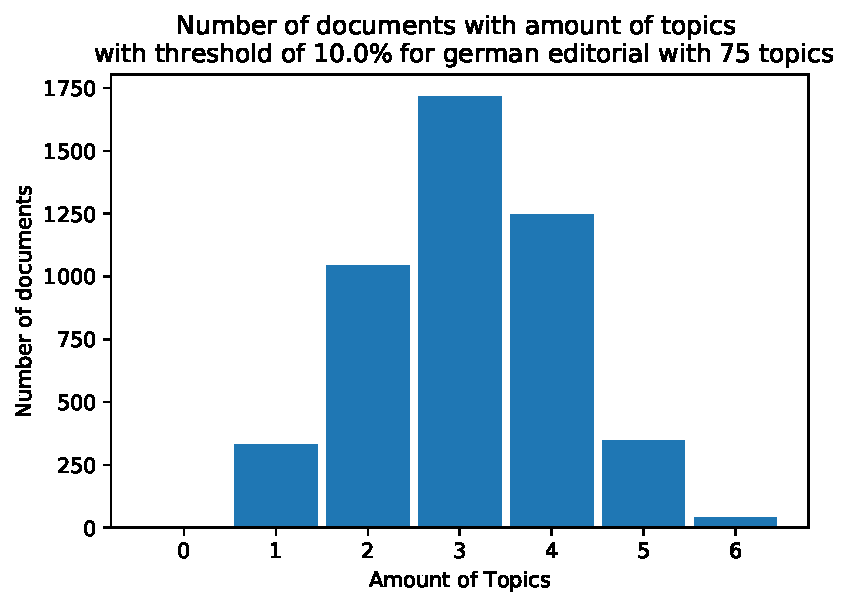
\includegraphics[width=7cm]{gfx/GrafikenFinal/germaneditoriallda_topPerdoc75.pdf}
	\end{minipage}
	\begin{minipage}[t]{0.5\textwidth}
		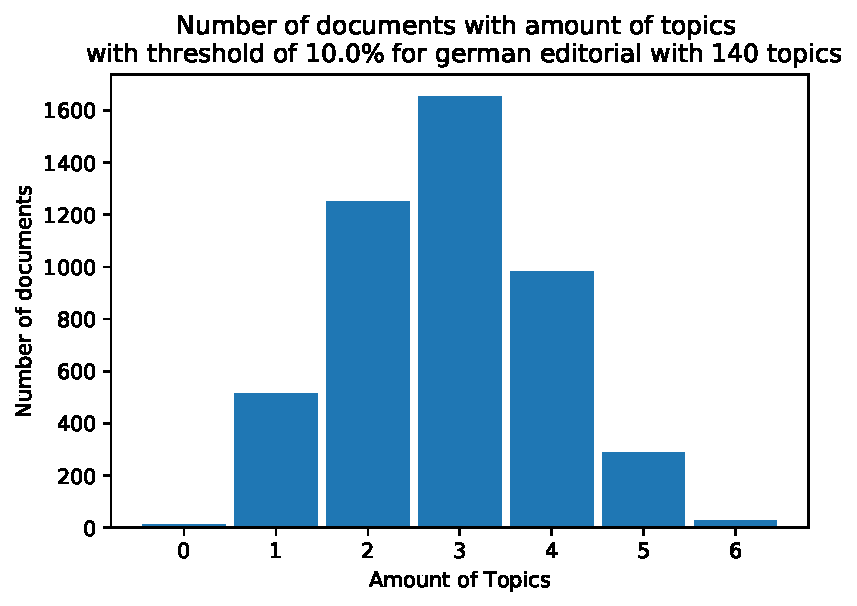
\includegraphics[width=7cm]{gfx/GrafikenFinal/germaneditoriallda_topPerdoc140.pdf}
	\end{minipage}
	\begin{minipage}[t]{0.5\textwidth}
		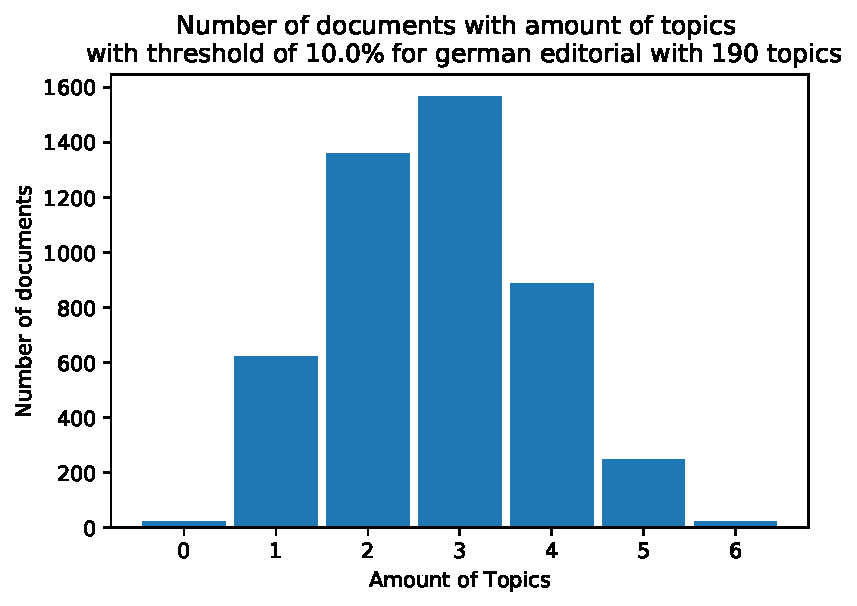
\includegraphics[width=7cm]{gfx/GrafikenFinal/germaneditoriallda_topPerdoc190.pdf}
	\end{minipage}
	\begin{minipage}[t]{0.5\textwidth}
		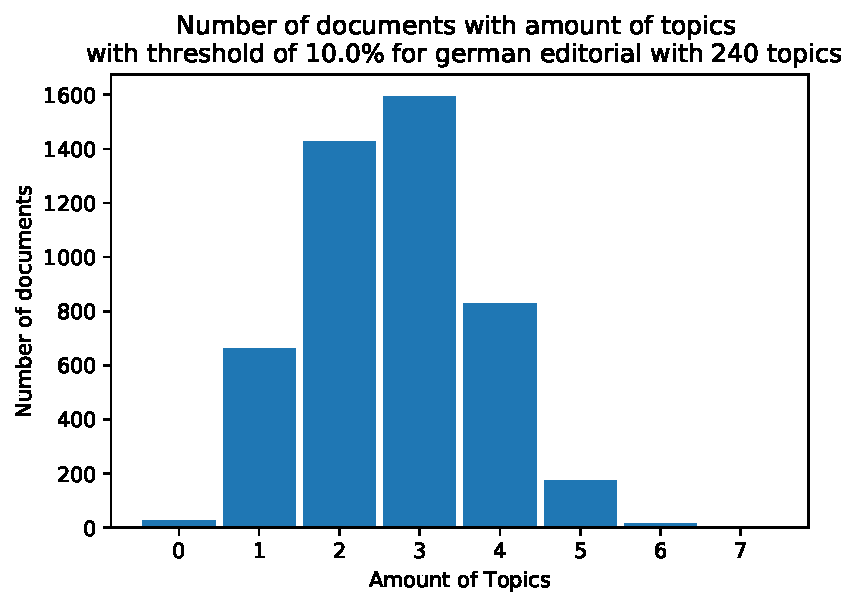
\includegraphics[width=7cm]{gfx/GrafikenFinal/germaneditoriallda_topPerdoc240.pdf}
	\end{minipage}
	\caption[]{Amount of topics in documents over a threshold of 10\% for German editorial articles}
	\label{top_per_doc_ger}
\end{figure}

Second, we analyzed how many topics occur in a document over 10\%. 
The plots in Figure \ref{top_per_doc_ger} and \ref{top_per_doc_eng} represent the number of documents with the number of topics over the threshold. On the x-axis the amount of topics, which are occurring over 10\%in a document, while the y-axis represents the number of documents, which include a certain amount of topics. 

In Figure \ref{top_per_doc_eng} is shown how the number of topics for \textit{English editorial articles} change. When increasing the number from 25 to 50 topics, all documents are modeled by a most 6 topics. This means, that with a higher topic number the topics are more tailored to documents and thus the documents can be represented with less topics. This is also supported by the observation, that the number of documents, that contain only one or two topics over the threshold are slightly increasing with the number of topics. At the same time there are some documents, that do not express any topic over the threshold, which could indicate, that these documents are rather general and cover many topics with a low probability, instead of covering a few specific topics.
 %Across all plots the maximal number of topics, occurring in a document is 3 and does not change. Only the number of documents decreases from above 850 documents to about 780 documents. From the plots with 130 to 180 topics no significant changes can be seen. One can deduce from the plots, that the topics are getting more specific. 
For the \textit{German editorial articles} in Figure \ref{top_per_doc_ger} it can be seen, that the maximal number of topics, covering a document is also at 3. From the topic model with 25 topics to 50 topics, there are no documents, which include 8 topics, but there are documents, that do not contain any topic. When increasing the number of topics to the next level, there are no documents, which contain 7 topics. In the next plots, the number of documents containing 2, only 1 or no topic is raising, but the maximal topic number remains 3. The last plot is looking nearly the same apart from adding a few documents with 7 topics. For this dataset it could be said, that the topics are getting up to 190 topics more specific. With more topics the number of generic topics increases. So the topic model with 190 seems the best for obtaining good topics.


\subsubsection{Jensen Shannon divergence}

The \ac{JS} divergence was used to calculate the similarity of topics based on the topic term matrix in a topic model and across topic models. The similarities were then visualized as heat maps. The dark red colored boxes express high similarity, while the brighter boxes express a smaller similarity.  
The topic models form \textit{German editorial articles} with 25, 50 and 70 topics were evaluated manually. The highest similarities (dark red) with the values of 0.63, 0.65, and 0.65 for the topics intra a topic model were taken, and the topics were compared with each other in Table \ref{intra_topic}. The same words form the top 10 terms of a topic were marked in bold. In Table \ref{inter_topic} the similarities of the topics were calculated across different topic models with 25/50, 50/57 and 50/75 topics. The values for the similarity were 0.9, 0.87 and 0.94. One can see, that the number of common words and the calculated similarity, is much higher in the inter topic model evaluation. This means, that the topics inter a topic model are not as similar to each other as the topics developing across topic models. At least this is not recognizable by the top 10 words of a topic. The heat maps for the inter topic model and intra topic model evaluation can be seen in Figure \ref{heatmap:inter_ger} and \ref{heatmap:intra_ger}.
%TODO heatmaps in anhang

Within the different topic models the topics are hardly similar. This is a good characteristic, because it shows, that the topic number was not over fitted. Across the topic models there are different topics, but also very similar topics, which is shown in Table \ref{min_max_sim_ger} for \textit{German editorial articles} and in Table \ref{min_max_sim_eng} for \textit{English editorial articles}. This means, when increasing the number of topics, some of the new generated topics do not change much and cover the same themes such as the previous topic model, but new topics are added, too, which cover new themes. By adding new topics the development of the topics can be tracked. 


\begin{table}
	\centering
	\begin{tabular}{c|c|c}
		topics& \multicolumn{2}{c}{compared topics with the highest similarity:}\\
		\hline
		25 & T1:\thead{all, jed, sehen,\\ stehen, leben, einfach, welt,\\finden, frage, bio}&T19:\thead{bauer, landwirt, landwirtschaft,\\ milch, preisen, kuh, betrieb,\\ hof, euro, cent}\\
		\hline
		50 &T42:\thead{essen, lebensmittel, \textbf{jed},\\ fleich, all, kaufen, leben,\\ \textbf{stehen}, ernährung, einfach}&T40:\thead{hof, betreiben, landwirtschaft,\\ \textbf{stehen}, landwirt, bauer, familie,\\ verkaufen, \textbf{jed}, alt}\\
		\hline
		75&T63:\thead{bauer, landwirt, euro,\\ \textbf{preisen}, konventionell, biobauer, geld, \\bekommen, umstellen, ernten}&T67:\thead{product, verbraucher, kunde,\\ deutschland, \textbf{preisen}, deutsch, prozent,\\ handeln,supermarkt, deutsche}
	\end{tabular}
	\caption[]{Compared topics intra a topic model with the highest similarity. Common topic words are \textbf{bold}}
	\label{intra_topic}
\end{table}

\begin{table}
	\centering
	\begin{tabular}{c|c|c}
		topics& \multicolumn{2}{c}{compared topics with the highest similarity:}\\
		\hline
		25/50 & T21:\thead{\textbf{prozent}, \textbf{euro}, \textbf{ökologisch}, \textbf{betrieb},\\ \textbf{hektar}, million, steigen,\\ \textbf{fläche}, deutschland, \textbf{zahlen}}&
			T2:\thead{\textbf{prozent}, \textbf{ökologisch}, \textbf{betrieb}, \textbf{hektar},\\ \textbf{fläche}, landwirtschaft, \textbf{zahlen},\\ anteil, bewirtschaften, \textbf{euro}}\\
			\hline
			50/75 &T4:\thead{\textbf{pestizid}, \textbf{finden}, \textbf{probe}, \textbf{rückstand},\\ \textbf{greenpeace}, konventionell, \textbf{untersuchen}, \\\textbf{belasten}, prozent,einsatz}&T54:\thead{\textbf{pestizid}, \textbf{rückstand}, \textbf{probe}, grenzwert,\\ \textbf{finden}, \textbf{greenpace}, stoff,\\ \textbf{belasten}, \textbf{untersuchen}, einsetzen}\\ 
			\hline
			50/75&T9:\thead{\textbf{eiern}, \textbf{fipronil}, \textbf{belasten}, \textbf{niederlande},\\ \textbf{deutschland}, \textbf{nehmen}, \textbf{verkaufen},\\\textbf{betreffen}, betrieb, angeben}&T57:\thead{\textbf{eiern}, \textbf{fipronil}, \textbf{belasten}, \textbf{niederlande},\\ \textbf{nehmen}, \textbf{deutschland}, \textbf{verkaufen}, \\betroffen, \textbf{betreffen}, behörde}\\
		\end{tabular}
		\caption[]{Compared topics inter topic models with the highest similarity. Common topic words are \textbf{bold}}
		\label{inter_topic}
\end{table}

\begin{figure}
	\begin{minipage}[t]{0.5\textwidth}
		\subfloat[Minimal and maximal similarities for German editorial articles inter different topic models]{
		\begin{tabular}{c|c|c}
			topics & min value &max value\\
			\hline
			25&0.38&0.63\\
			50& 0.35 & 0.65\\
			75&0.33&0.65\\
			140&0.34&0.62\\
			190&0.33&0.61\\
			240&0.33&0.60\\
		\end{tabular}}
	\end{minipage}
	\begin{minipage}[t]{0.5\textwidth}
		\subfloat[Minimal and maximal similarities for German editorial articles intra different topic models]{
		\begin{tabular}{c|c|c}
			topics & min value &max value\\
			\hline
			25/50&0.35&0.91\\
			25/75& 0.35 & 0.88\\
			50/75&0.35&0.94\\
			140/190&0.33&0.88\\
			140/240&0.32&0.92\\
			190/240&0.33&0.91\\
		\end{tabular}}
	\end{minipage}
\caption[]{Minimal and maximal similarities inter and intra topic models for German editorial articles}
\label{min_max_sim_ger}
\end{figure}


\begin{figure}
	\begin{minipage}[t]{0.5\textwidth}
		\subfloat[Minimal and maximal similarities for English editorial articles inter different topic models]{
			\begin{tabular}{c|c|c}
				topics & min value &max value\\
				\hline
				25&0.42&0.66\\
				50& 0.36 & 0.68\\
				75&0.35&0.69\\
				80&0.35&0.67\\
				130&0.34&0.65\\
				180&0.36&0.67\\
			\end{tabular}
			}
	\end{minipage}
	\begin{minipage}[t]{0.5\textwidth}
		\subfloat[Minimal and maximal similarities for English editorial articles intra different topic models]{
		\begin{tabular}{c|c|c}
			topics & min value &max value\\
			\hline
			25/50&0.39&0.90\\
			25/75& 0.37 & 0.91\\
			50/75&0.35&0.91\\
			80/130&0.34&0.95\\
			80/180&0.33&0.97\\
			130/180&0.33&1.0\\
		\end{tabular}}
	\end{minipage}
	\caption{Minimal and maximal similarities inter and intra topic models for English Editorial articles}
	\label{min_max_sim_eng}
\end{figure}



\subsubsection{Correlation}
Calculating the correlation between every key figure, the relationship over the different topic models is analyzed by using the Pearson correlation. It is a measure of the linear correlation between two variables $X$ and $Y$ and can assume values between 1 an -1, where 1 represents a total positive linear correlation, 0 no linear correlation and -1 represents a total negative linear correlation. 

In Figure \ref{Corr} the correlation for the key figures alpha, entropy, coherence and documents per topic is calculated. 
On the x-axis the topic models with different topics is shown, while the y-axis shows the calculated correlation.

One can see, that the alpha and documents per topic values are correlating. This is, because both 
measure the sparsity of a topic over documents in a corpus. The alpha values, coherence values and documents
per topic values hardly correlate. From this one can deduce, that the topics, which are most present 
in a document are not so easily interpretable for humans. Furthermore, all correlations including 
entropy are at the beginning highly correlating, but the correlation coefficient is continuously decreasing. 
So entropy in general seem to be a metric, which is developing independently form the other key
figures, so from the characteristic, if a topic is rather general or specific, can not be deduced, 
if the topic is strongly represented in a document or if it is easily interpretable.

\begin{figure}
	\begin{minipage}[t]{0.5\textwidth}
	\subfloat[Correlation for German editorial articles]{
	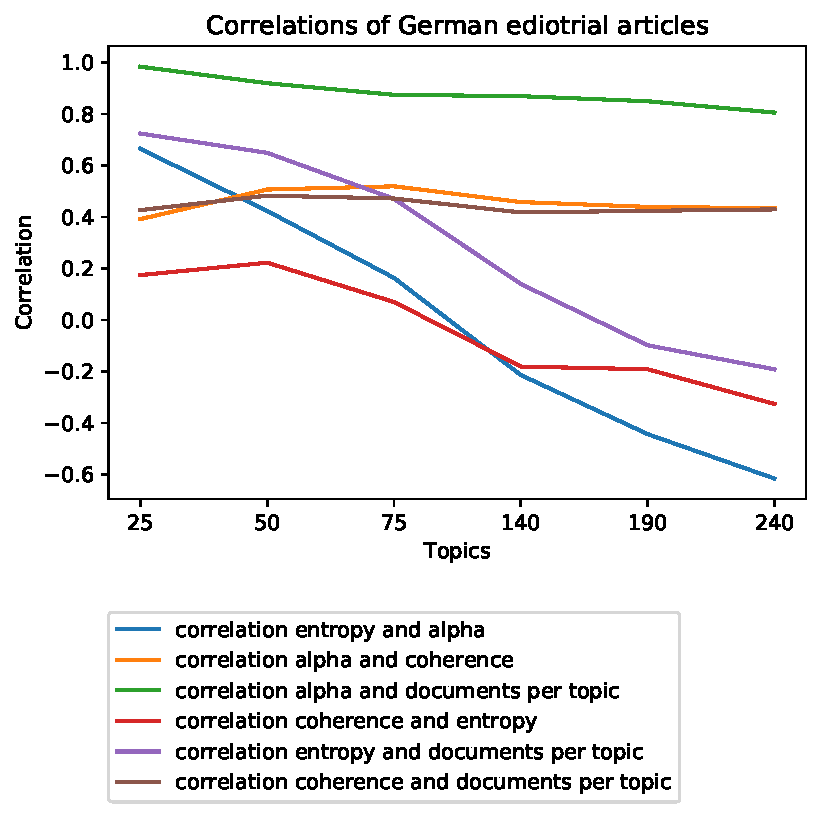
\includegraphics[width=7cm]{gfx/Correlation/6Cor_germ.pdf}}
	\end{minipage}
	\begin{minipage}[t]{0.5\textwidth}
		\subfloat[Correlation for English editorial articles]{
	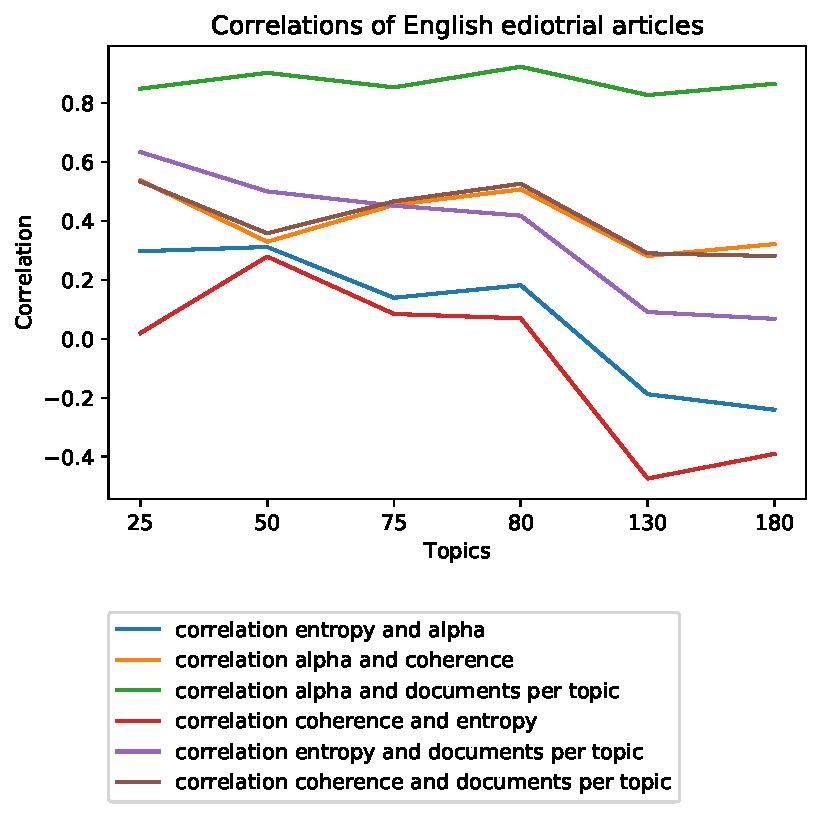
\includegraphics[width=7cm]{gfx/Correlation/6Cor_eng.pdf}}
	\end{minipage}
\caption[]{Correlations of key figures for German and English editorial articles}
\label{Corr}
\end{figure}

The analysis of the different key figures on the two datasets has shown that no key figure on its own is enough to determine the quality or the optimal topic number. When considering multiple key figures, it is possible to compare different topic models based on how generic or specific the topics are (entropy) or how the topics are distributed across the corpus (alpha). It is not possible, however, to compare topic models of different datasets. Each dataset has its own characteristics such as the number of documents, the average length of the documents or how specific the topics are covered. These differences make it impossible to compare topic models trained on different datasets. 

%resume: besten kriterien lassen sich nicht so leich bestimmen. da es vom datensatz abhägen kann, aus wie vielen dokumenten besteht der corpus, wie lang sind diese documente. und wie spezifisch sind die themen, die in einem document behandelt werden.



\newpage